This chapter consists of two sections, the first one shows an overview some of the
different methods that have been previously used in the literature
for understanding or estimating urban perception, these methods are separated
into 3 types: the classic approaches (all the methods not relying on
massive amounts of data are grouped here), approaches based on machine learning and
approaches consisting of machine learning models combined with other techniques.
The different methods are explained and a brief analysis of advantages and disadvantages
is provided for each of them. Section two summarizes the main aspects of the research
on explainability on deep learning, and describes some techniques that have been applied
in urban perception or other domains that are relevant for this work.


\section{Solutions for estimating urban perception.}

\subsection{Classic approaches.}
Methods for measuring perception of urban spaces have appeared in the literature of several
disciplines for many years,  with some of the most influential studies dating back to 1960
\cite{lynch}. Due to technological limits the literature consisted mainly of several types of
qualitative surveys for a long time. This surveys consisted in having subjects, complete
different tasks such as drawing maps of a certain place \cite{lynch}, evaluating fundamental
aspects of a neighborhood \cite{nasar_perception}, or in more recent approaches evaluating
the impact of transformations generated with edited images \cite{jiang_minimizing}. Most of
these surveys were conducted in person or by phone, and then the results were analyzed manually,
making it very difficult and costly to scale to multiple locations, or larger amounts of samples.
The main benefit of this approach, is that it permits a very refined control of the observation process
since both the subjects being interviewed and the spaces in question are chosen by the researcher.
Added to that, the experiments conducted in person allow for the observer to use senses different
than vision to analyze the subject space, resulting in a richer appreciation.

Other methodology, more common in economics and engineering, consists of using discrete choice models
and stated choice surveys to model the effect of different variables in perception or other urban
related variables  \cite{rose_sc, iglesias_perception, torres_housing}. The amount and complexity of the
variables measured depends on the model design. To have and exact control of the variables that
have an effect on the survey, computer generated images of urban spaces can be used
\cite{iglesias_perception,torres_housing}.

The advantage of this method is that through the estimated parameters of the model, the effect
of each of the studied variables on the perception estimation can be measured, allowing for
quantitative results and an understanding of the impact different elements have on the
perception of the urban landscape. The main disadvantage of this approach comes from the
difficulty of the  survey design, variables need to be chosen carefully and the process its
vulnerable to biases from the model designer.

\subsection{Pure machine learning approaches.}

Thanks to the massive adoption of web and mobile technologies such as google maps, new types of
data are available in considerably large volumes, and new highly scalable ways of  generating data can be
designed and implemented quickly. That fact allows for some very data dependent machine learning
algorithms to be applied to new  problems, including urban perception estimation. Several different
datasets have been proposed for this problem, most of them based on surveys over large amounts of urban images
\cite{hidalgo_inequality, hidalgo_placepulse, quercia_aesthetic, liu_machine, santani}. The most important
of them, all consisting of pairwise comparisons of street view images, are \textit{Place pulse 1.0} (PP 1) \cite{hidalgo_inequality}
with measures of safety, class and uniqueness over images of 4 cities, \textit{Urban Gems} with measures of
beauty, quietness and happiness over images of London and \textit{Place pulse 2.0} (PP 2) \cite{hidalgo_placepulse}, the largest dataset
available, with measures of six different attributes over images of 56 different cities, the models proposed on this work are
trained on this dataset. All of these were collected through public online surveys of large scale, where the users
are asked to choose the image most representative of an attribute of a pair, see figure \ref{fig:survey} for an example.

\begin{figure}[ht]
	\begin{center}
	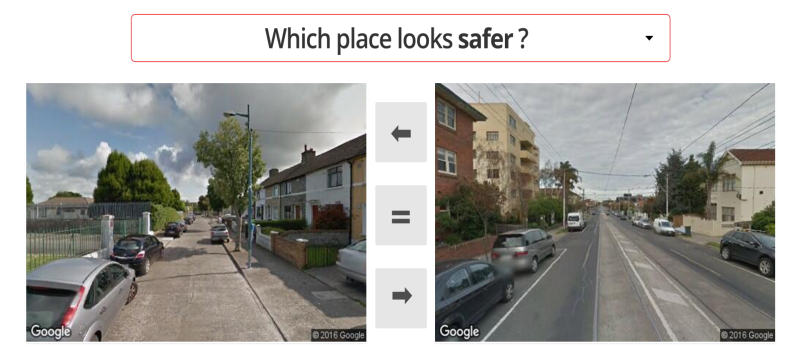
\includegraphics[width=0.5\textwidth]{./figures/placepulse.png}
	\caption[Place pulse 2.0 survey]{Snapshot of the place pulse 2.0 survey. Extracted from \citeA{hidalgo_placepulse} }
	\label{fig:survey}
	\end{center}
\end{figure}

Earlier attempts at using this data for training models tried to turn the problem into a classification problem
by  ranking the images from the votes with manually engineered methods such as the one suggested on the
place pulse 1.0 paper \cite{hidalgo_inequality} and use the rank to split the data in two halves with a different
label, \citeA{tamara_judgments} use this approach to train SVM models on PP 1 using different types of visual features as input,
including a deep neural network. On the PP 2 paper, the authors present the first end to end deep learning model for
urban perception regression, which uses a typical transfer learning technique \cite{survey_transfer}, a
Imagenet \cite{imagenet} pretrained  network for the base of the model, which is used as input
for by two parallel modules, one for classification and one for regression. They train the architecture
separately on the 6 different attributes of the dataset, the models learn to emulate human voting and
to output a urban perception score (through the regression module) on the image for the correspondent attribute.

\subsection{Mixed approaches.}

\section{ Explainability in deep learning.}